
\chapter[Lý thuyết: Sóng dừng]{Lý thuyết: Sóng dừng}
\section{Lý thuyết}
\subsection{Sự phản xạ của sóng}
\subsubsection{Phản xạ của sóng trên vật cản cố định}
Khi phản xạ trên vật cản cố định, sóng phản xạ luôn ngược pha với sóng tới ở điểm phản xạ.
\begin{center}
	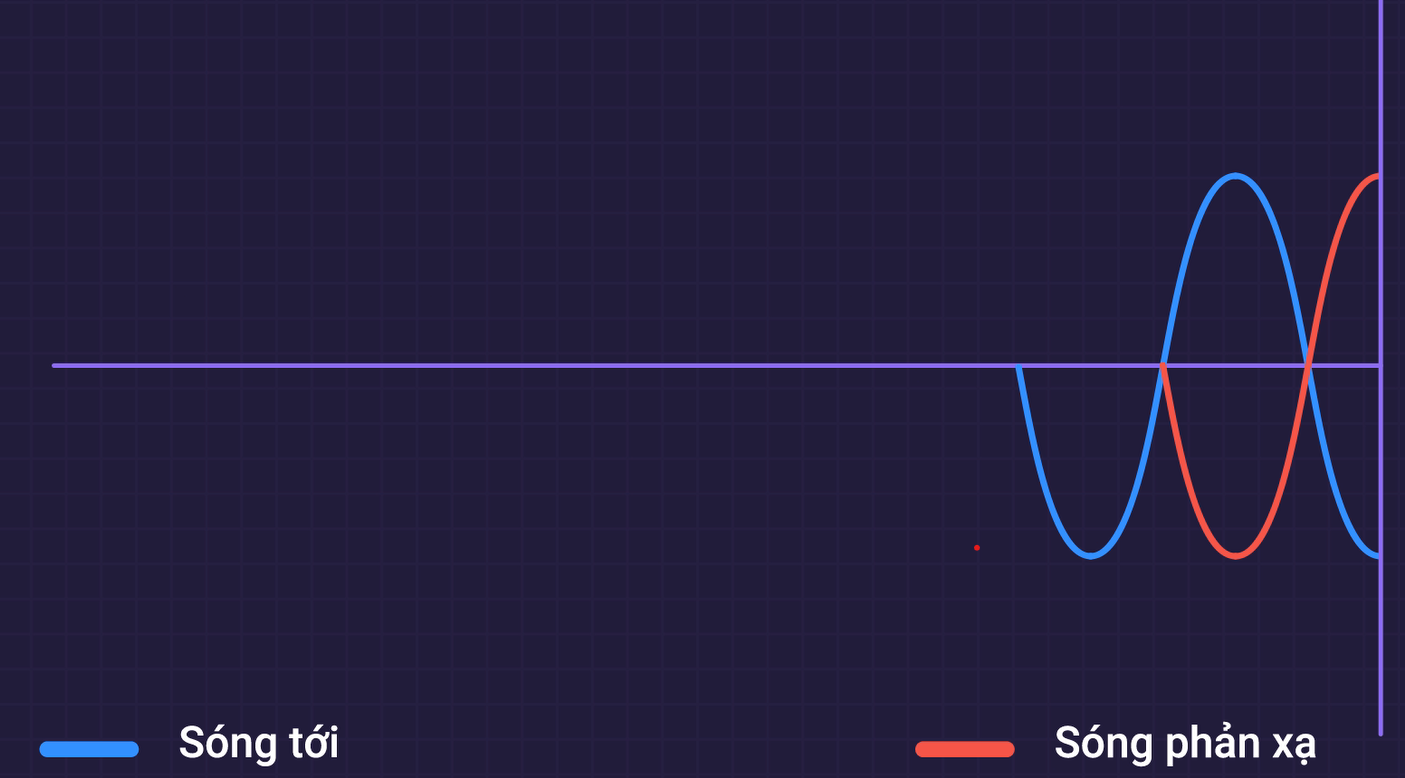
\includegraphics[scale=0.3]{../figs/VN12-PH-12-L-007-1-V2-1.png}
\end{center}
\subsubsection{Phản xạ của sóng trên vật cản tự do}		
Khi phản xạ trên vật cản tự do, sóng phản xạ luôn cùng pha với sóng tới ở điểm phản xạ.
\begin{center}
	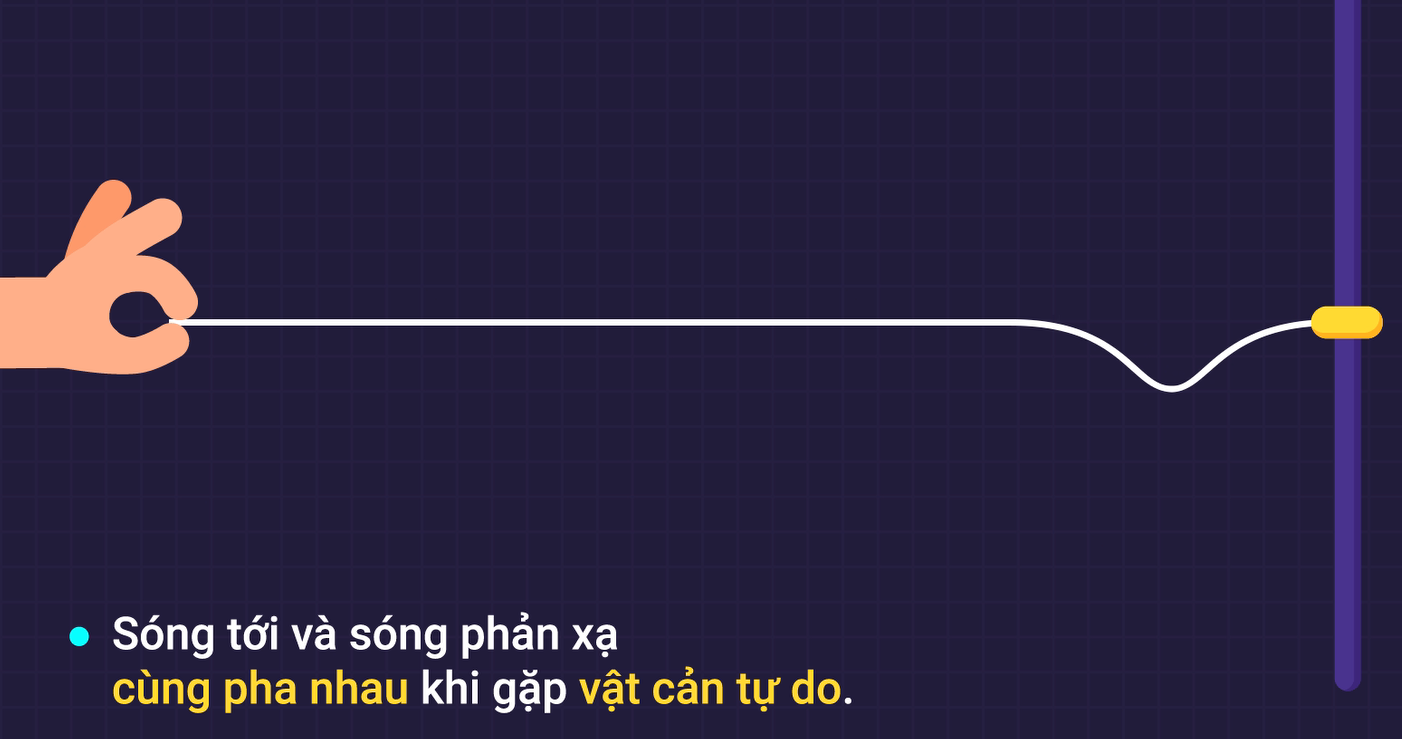
\includegraphics[scale=0.3]{../figs/VN12-PH-12-L-007-1-V2-2.png}
\end{center}
\subsection{Sóng dừng}
\subsubsection{Hiện tượng }
Sóng tới và sóng phản xạ, nếu truyền theo cùng một phương, thì có thể giao thoa với nhau và tạo thành một hệ sóng dừng.
\begin{center}
	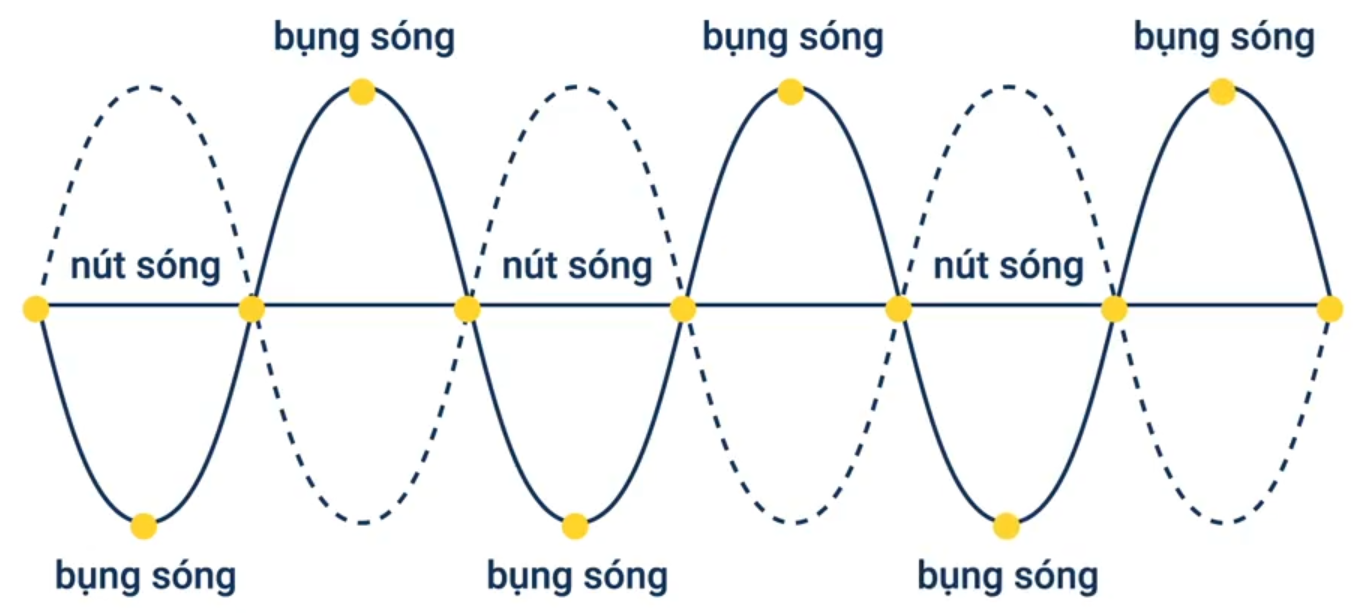
\includegraphics[scale=0.3]{../figs/VN12-PH-12-L-007-1-V2-3.png}
\end{center}	
\subsubsection{Đặc điểm}
\begin{itemize}	
	\item Trong sóng dừng, có một số điểm luôn đứng yên gọi là nút sóng và một số điểm luôn dao động với biên độ cực đại gọi là bụng sóng. 
	\item Khoảng cách giữa hai nút liên tiếp hoặc hai bụng liên tiếp bằng nửa bước sóng.
	\item Với sóng dừng trên dây, đầu cố định luôn là nút sóng, đầu tự do luôn là bụng sóng.
\end{itemize}
\begin{center}
	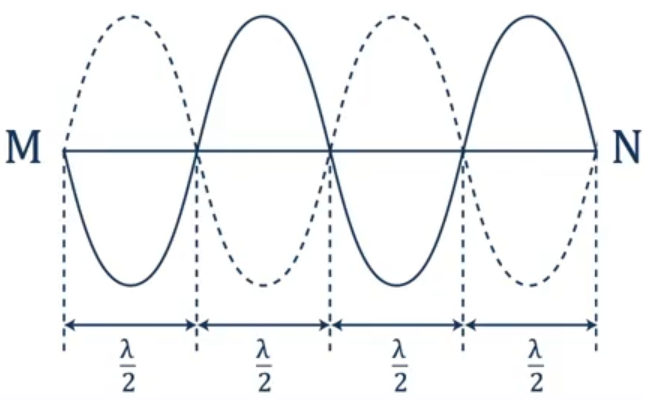
\includegraphics[scale=0.6]{../figs/VN12-PH-12-L-007-1-V2-4.png}
\end{center}
\section{Mục tiêu bài học - Ví dụ minh họa}
\begin{dang}{Ghi nhớ được định nghĩa sóng dừng}
	\viduii{1}
	{Sóng dừng là
		\begin{mcq}
			\item sóng không lan truyền được do bị một vật cản chặn lại.
			\item sóng được tạo thành giữa hai điểm cố định trong một môi trường.
			\item sóng được tạo thành do sự giao thoa giữa sóng tới và sóng phản xạ.
			\item sóng được tạo thành do sự giao thoa của hai sóng kết hợp, trên đường thẳng nối giữa hai tâm phát sóng.
		\end{mcq}
	}
	{
		\begin{center}
			\textbf{Hướng dẫn giải}
		\end{center}
		
		Sóng tới và sóng phản xạ, nếu truyền theo cùng một phương, thì có thể giao thoa với nhau và tạo thành một hệ sóng dừng.
		
		\textbf{Đáp án: C.}
	}
	\viduii{1}
	{Ta quan sát được hiện tượng gì trên sợi dây có sóng dừng?
		
		\begin{mcq}
			\item Tất cả các phần tử trên dây đều đứng yên.
			\item Trên dây có những bụng sóng xen kẽ với nút sóng.
			\item Tất cả các điểm trên dây đều dao động với biên độ cực đại.
			\item Tất cả các điểm trên dây đều chuyển động với cùng tốc độ.
		\end{mcq}
	}
	{\begin{center}
			\textbf{Hướng dẫn giải}
		\end{center}
		
		Trong sóng dừng, có một số điểm luôn đứng yên gọi là nút sóng và một số điểm luôn dao động với biên độ cực đại gọi là bụng sóng.
		
		\textbf{Đáp án: B.}
	}
\end{dang}
\begin{dang}{Mô tả được sự phản xạ của sóng\\ trên vật cản cố định, vật cản tự do}
	\viduii{1}
	{Chọn câu đúng. Tại điểm phản xạ thì sóng phản xạ
		\begin{mcq}
			\item luôn ngược pha với sóng tới.
			\item ngược pha với sóng tới nếu vật cản là cố định.
			\item ngược pha với sóng tới nếu vật cản là tự do. 
			\item cùng pha với sóng tới nếu vật cản là cố định.
		\end{mcq}
	}
	{
		\begin{center}
			\textbf{Hướng dẫn giải}
		\end{center}
		
		Nếu sóng tới gặp một vật cản cố định thì tại điểm phản xạ, sóng phản xạ ngược pha với sóng tới.
		
		\textbf{Đáp án: B.}
	}
	\viduii{1}
	{Khi nói về sự phản xạ của sóng cơ trên vật cản cố định, phát biểu nào sau đây đúng?
		
		\begin{mcq}
			\item Tần số của sóng phản xạ luôn lớn hơn tần số của sóng tới. 
			\item Sóng phản xạ luôn ngược pha với sóng tới ở điểm phản xạ. 
			\item Tần số của sóng phản xạ luôn nhỏ hơn tần số của sóng tới. 
			\item Sóng phản xạ luôn cùng pha với sóng tới ở điểm phản xạ. 
		\end{mcq}
	}
	{\begin{center}
			\textbf{Hướng dẫn giải}
		\end{center}
		
		Nếu sóng tới gặp một vật cản cố định thì tại điểm phản xạ sóng tới ngược pha với sóng phản xạ.
		
		\textbf{Đáp án: B.}
	}
\end{dang}
\begin{dang}{Giải thích được hiện tượng sóng dừng}
	\viduii{1}
	{Khi có sóng dừng trên một sợi dây đàn hồi thì khoảng cách giữa hai bụng sóng liên tiếp bằng
		\begin{mcq}(4)
			\item $2\lambda$.
			\item $\lambda$. 
			\item $\dfrac{\lambda}{4}$.
			\item $\dfrac{\lambda}{2}$.
		\end{mcq}
	}
	{
		\begin{center}
			\textbf{Hướng dẫn giải}
		\end{center}
		
		Khi có sóng dừng trên một sợi dây đàn hồi thì khoảng cách giữa hai bụng sóng liên tiếp bằng nửa bước sóng ($\dfrac{\lambda}{2}$).
		
		\textbf{Đáp án: D.}
	}
	\viduii{2}
	{Khi có sóng dừng trên một sợi dây đàn hồi thì khoảng cách từ một bụng đến một nút gần nó nhất bằng
		
		\begin{mcq}(4)
			\item $2\lambda$.
			\item $\lambda$. 
			\item $\dfrac{\lambda}{4}$.
			\item $\dfrac{\lambda}{2}$.
		\end{mcq}
	}
	{\begin{center}
			\textbf{Hướng dẫn giải}
			
			\vspace*{1em}
			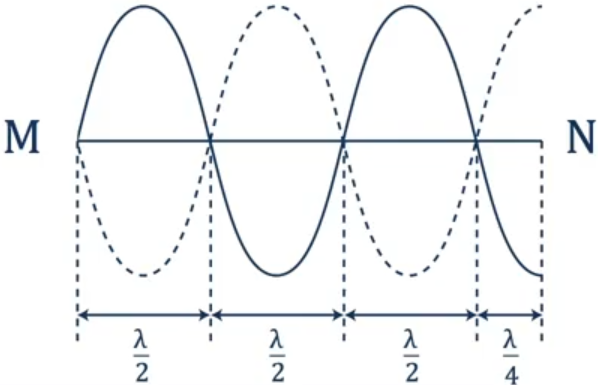
\includegraphics[scale=0.6]{../figs/VN12-PH-12-L-007-1-V2-5.png}
		\end{center}
		
		Khi có sóng dừng trên một sợi dây đàn hồi thì khoảng cách từ một bụng đến một nút gần nó nhất bằng một phần hai của một nửa bước sóng, tức là $\dfrac{\lambda}{4}$.
		
		\textbf{Đáp án: C.}
	}
\end{dang}